\documentclass{article}
\usepackage[utf8]{inputenc}
% \usepackage[english,greek]{babel}
\usepackage[unicode]{hyperref}
\usepackage[LGR, T1]{fontenc}
\usepackage{amsfonts, alphabeta, amssymb}
\usepackage[none]{hyphenat}
\usepackage{amsmath, slashed, graphicx, physics, tikz, braket, caption, subfig, comment, geometry, multicol, lipsum, fancyhdr, tcolorbox, siunitx, authblk, xcolor, abstract, float, indentfirst, xfrac, cancel, bbold, appendix, tikz, tikz-feynman, tensor, multirow, makecell, algpseudocode, algorithmicx, algorithm, changepage, adjustbox, lscape, placeins}
\usepackage[style=numeric-comp,sorting=none]{biblatex}
\addbibresource{references.bib}
\setcounter{secnumdepth}{3}
\setcounter{tocdepth}{3}
\title{\textbf{
        Study of a new kinematic weighting algorithm for the measurement of CP asymmetries in charm decays}
        \\
        LHCb Collaboration
}
\author{
        Georgios Christou
        \\
        Supervisors: Dr.\@ Federico Betti, Prof.\@ Angelo Carbone
}
\date{
        August 2023
}

\begin{document}
        \begin{figure}[t]
                \centering
                \subfloat{
\includegraphics[height = 3.5cm]{../.images/CERN_logo.png}}
                \hspace{1cm}
                \subfloat{
\includegraphics[height = 3.5cm]{../.images/Lhcb-logo-new.svg.png}}
        \end{figure}

        \maketitle

        \begin{abstract}
                We investigate the asymmetries that occur in charm decays at the LHCb, specifically we study $D^{\star+}\to D^0\pi^+$ and $\bar{D}^{\star-}\to D^0\pi^-$ where $D^0\to K^-K^+$ or $D^0\to \pi^-\pi^+$.
                We study the effect of $CP$ and detection asymmetries on MC samples generated via RapidSim and implement a new kinematic weighting function which allows us to keep events that are otherwise discarded from LHCb data, since they are associated with large detection asymetries.
        \end{abstract}
        
        \pagebreak
        % \tableofcontents
        % \pagebreak

        \section{Introduction}
        We investigate charm decays and specifically the $D^\star$ meson.
        By studying the differences between $D^{\star +}$ and $D^{\star -}$ decays shown in Fig. \ref{fig:diagrams} we can estimate the $CP$ asymmetry in charm decays.
        \begin{figure}[h!]
                \centering
                \subfloat{
                        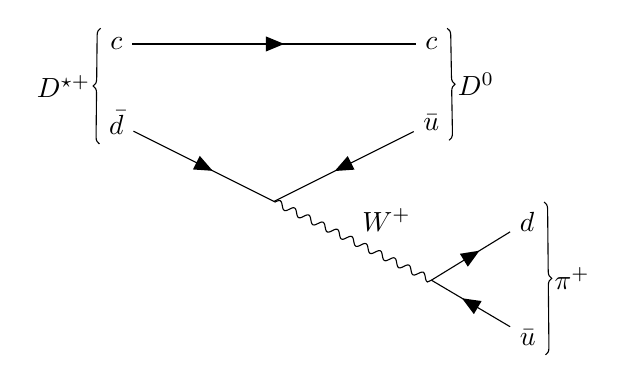
\begin{tikzpicture}
                                \begin{feynman}
                                        \vertex (DStarC) {$c$};
                                        \vertex[below = 1cm of DStarC] (DStarDBar) {$\bar{d}$};

                                        \vertex[right = 4cm of DStarC] (D0C) {$c$};
                                        \vertex[right = 4cm of DStarDBar] (D0UBar) {$\bar{u}$};

                                        \vertex[below right = 1cm and 2cm of DStarDBar] (WStart);
                                        \vertex[below right = 1cm and 2cm of WStart] (WEnd);

                                        \vertex[above right = 0.5cm and 1cm of WEnd] (PiD) {$d$};
                                        \vertex[below right = 0.5cm and 1cm of WEnd] (PiUBar) {$\bar{u}$};
                                        \diagram*{
                                                (DStarC) -- [fermion] (D0C);
                                                (DStarDBar) -- [fermion] (WStart);
                                                (D0UBar) -- [fermion] (WStart);
                                                (WStart) -- [photon, edge label = $W^+$] (WEnd);
                                                (PiUBar) -- [fermion] (WEnd);
                                                (WEnd) -- [fermion] (PiD);
                                        };
                                        \draw [decoration={brace}, decorate] (DStarDBar.south west) -- (DStarC.north west) node [pos=0.5, left] {$D^{\star +}$};
                                        \draw [decoration={brace}, decorate] (D0C.north east) --  (D0UBar.south east) node [pos=0.5, right] {$D^0$};
                                        \draw [decoration={brace}, decorate] (PiD.north east) --  (PiUBar.south east) node [pos=0.5, right] {$\pi^+$};
                                \end{feynman}
                        \end{tikzpicture}
                }
                \subfloat{
                        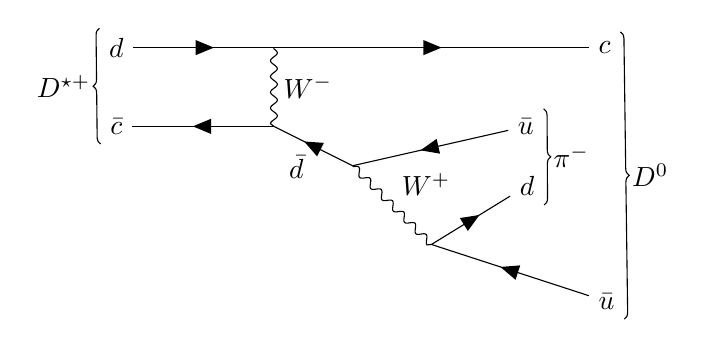
\begin{tikzpicture}
                                \begin{feynman}
                                        \vertex (DStarD) {$d$};
                                        \vertex[below = 1cm of DStarD] (DStarCBar) {$\bar{c}$};

                                        \vertex[right = 6.2cm of DStarD] (D0C) {$c$};
                                        \vertex[right = 5.2cm of DStarCBar] (D0UBar) {$\bar{u}$};

                                        \vertex[right = 2cm of DStarD] (WMinusStart);
                                        \vertex[right = 2cm of DStarCBar] (WMinusEnd);

                                        \vertex[below right = 0.5cm and 1cm of WMinusEnd] (mid);

                                        \vertex[below right = 1cm and 1cm of mid] (W);

                                        \vertex[above right = 0.5cm and 1cm of W] (PiD) {$d$};
                                        \vertex[below right = 0.5cm and 2cm of W] (PiUBar) {$\bar{u}$};

                                        \diagram*{
                                                (DStarD) --[fermion] (WMinusStart);
                                                (WMinusStart) --[fermion] (D0C);
                                                (WMinusStart) --[photon, edge label = $W^-$] (WMinusEnd);
                                                (D0UBar) --[fermion] (mid);
                                                (mid) --[fermion, edge label = $\bar{d}$] (WMinusEnd);
                                                (WMinusEnd) --[fermion] (DStarCBar);
                                                (mid) --[photon, edge label = $W^+$] (W);
                                                (PiUBar) -- [fermion] (W);
                                                (W) -- [fermion] (PiD);
                                        };
                                        \draw [decoration={brace}, decorate] (DStarCBar.south west) -- (DStarD.north west) node [pos=0.5, left] {$D^{\star +}$};
                                        \draw [decoration={brace}, decorate] (D0C.north east) --  (PiUBar.south east) node [pos=0.5, right] {$D^0$};
                                        \draw [decoration={brace}, decorate] (D0UBar.north east) --  (PiD.south east) node [pos=0.5, right] {$\pi^-$};
                                \end{feynman}
                        \end{tikzpicture}
                }
                \caption{Feynman diagram showing $D^{\star \pm}\to D^{0} \pi^{\pm}$ decays.}
                \label{fig:diagrams}
        \end{figure}

        The total asymmetry one observes at an experiment is a combination of multiple asymmetries.
        Namely, the total asymmetry consists of a \textit{CP asymmetry} and a \textit{detection asymmetry}.
        The former is associated with the difference between matter and anti-matter, while the latter is associated with the differences while detecting the soft pion $(\pi_s)$ that is produced during the decay.

        The total asymmetry can be estimated using 
        \begin{equation}
                \label{eq:total}
                A_\text{total} = \frac{A_{CP} + A_\text{D}}{1 + A_{C}A_\text{D}}
        \end{equation}
        where $A_{CP}$ and $A_\text{D}$ are the $CP$ and \textit{integrated detection asymmetries}.
        The latter can be calculated through
        \begin{equation}
                A_\text{D} = \frac{\int \dd \vec{p} N(\vec{p})A_\text{D}(\vec{p})}{\int dd \vec{p} N(\vec{p})}
        \end{equation}

        At the LHCb one observes large pion detection asymmetries that are associated with specific kinematic regions, which so far have been discarded, thus reducing the statistics.
        We can, however, introduce a \textit{weighting function} that allows us to keep events associated with large asymmetries.
        Such a weighting function can be expressed as the following ratio
        \begin{equation}
                \label{eq:weighting}
                Q(\vec{p}_{D^\star}, \vec{p}_{\pi_s}) \simeq \frac{\Gamma_{D^0}^{\pi\pi}(\vec{p}_{D^\star} - \vec{p}_{\pi_s}) + \Gamma_{\bar{D}^0}^{\pi\pi}(\vec{p}_{D^\star} - \vec{p}_{\pi_s})}{\Gamma_{D^0}^{KK}(\vec{p}_{D^\star} - \vec{p}_{\pi_s}) + \Gamma_{\bar{D}^0}^{KK}(\vec{p}_{D^\star} - \vec{p}_{\pi_s})}
        \end{equation}
        where $\Gamma_{D^{0}/\bar{D}^0}^{\pi\pi/KK}$ are the normalized distributions of $D^0$ candidates.
        Unfortunately in Run-2 such candidates were discarded, thus, we do not have a large enough sample to accurately calculate the weighting function, thus we resort to Monte Carlo simulations.

        
        \section{Analysis}
        \subsection{RapidSim}

        \pagebreak
        % \listoftables
        % \listoffigures
        \nocite{*}
        \printbibliography[notcategory=cited]
        \addcontentsline{toc}{chapter}{Bibliography}
\end{document}